% --- SLIDE 2: BIOMECHANICS ---
\begin{frame}{Biomechanics of Locomotion and Gait Dynamics}
    \begin{columns}[T]
        \begin{column}{0.45\textwidth}
            \begin{figure}
                \centering
                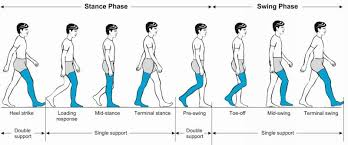
\includegraphics[width=\linewidth]{image/gait.jpeg}
                \caption{ Gait Cycle diagram (60\% Stance / 40\% Swing)}
            \end{figure}
            \vspace{-1.5em}
            \begin{block}{Froude Number ($Fr$)}
                \[ Fr = \frac{v^2}{g \cdot L} \]
                \centering \small Critical threshold $\approx 0.5$ for the walk-to-run transition.
            \end{block}
        \end{column}
        \begin{column}{0.55\textwidth}
            \begin{itemize}
                \item \textbf{Gait Cycle:} 
                \begin{itemize}
                    \item Transition between \textit{Stance Phase} (load absorption/push-off)
                    \item \textit{Swing Phase} (pendulum effect).
                \end{itemize}
                \item \textbf{Speed Parameters:} 
                \begin{itemize} 
                    \item Governed by \textit{Stride Length} 
                    \item \textit{Step Frequency}. Increasing frequency distributes the load over time. 
                \end{itemize}
                \item \textbf{Focus: Heel Strike \& Roll-over:}
                \begin{itemize}
                    \item Heel contact is the point of maximum stress at the \alert{residual limb–socket interface}.
                    \item Smooth roll-over is essential to minimize metabolic cost.
                \end{itemize}
                \item \textbf{Strategic Choice:} 
                \begin{itemize}
                    \item Cushioning localized at the heel. 
                    \item The forefoot remains rigid to ensure push-off (\textit{Toe-off}).
                \end{itemize}
            \end{itemize}
        \end{column}
    \end{columns}
\end{frame}